\documentclass[,jou, a4paper,floatsintext]{apa6}
\usepackage{lmodern}
\usepackage{amssymb,amsmath}
\usepackage{ifxetex,ifluatex}
\usepackage{fixltx2e} % provides \textsubscript
\ifnum 0\ifxetex 1\fi\ifluatex 1\fi=0 % if pdftex
  \usepackage[T1]{fontenc}
  \usepackage[utf8]{inputenc}
\else % if luatex or xelatex
  \ifxetex
    \usepackage{mathspec}
  \else
    \usepackage{fontspec}
  \fi
  \defaultfontfeatures{Ligatures=TeX,Scale=MatchLowercase}
\fi
% use upquote if available, for straight quotes in verbatim environments
\IfFileExists{upquote.sty}{\usepackage{upquote}}{}
% use microtype if available
\IfFileExists{microtype.sty}{%
\usepackage{microtype}
\UseMicrotypeSet[protrusion]{basicmath} % disable protrusion for tt fonts
}{}
\usepackage{hyperref}
\hypersetup{unicode=true,
            pdftitle={The Proportion of Signed Open Reviews Depends on the Recommendation},
            pdfauthor={Daniel Lakens~\& Nino van Sambeek},
            pdfkeywords={Peer Review, Open Science, Transparency},
            pdfborder={0 0 0},
            breaklinks=true}
\urlstyle{same}  % don't use monospace font for urls
\usepackage{graphicx,grffile}
\makeatletter
\def\maxwidth{\ifdim\Gin@nat@width>\linewidth\linewidth\else\Gin@nat@width\fi}
\def\maxheight{\ifdim\Gin@nat@height>\textheight\textheight\else\Gin@nat@height\fi}
\makeatother
% Scale images if necessary, so that they will not overflow the page
% margins by default, and it is still possible to overwrite the defaults
% using explicit options in \includegraphics[width, height, ...]{}
\setkeys{Gin}{width=\maxwidth,height=\maxheight,keepaspectratio}
\IfFileExists{parskip.sty}{%
\usepackage{parskip}
}{% else
\setlength{\parindent}{0pt}
\setlength{\parskip}{6pt plus 2pt minus 1pt}
}
\setlength{\emergencystretch}{3em}  % prevent overfull lines
\providecommand{\tightlist}{%
  \setlength{\itemsep}{0pt}\setlength{\parskip}{0pt}}
\setcounter{secnumdepth}{0}
% Redefines (sub)paragraphs to behave more like sections
\ifx\paragraph\undefined\else
\let\oldparagraph\paragraph
\renewcommand{\paragraph}[1]{\oldparagraph{#1}\mbox{}}
\fi
\ifx\subparagraph\undefined\else
\let\oldsubparagraph\subparagraph
\renewcommand{\subparagraph}[1]{\oldsubparagraph{#1}\mbox{}}
\fi

%%% Use protect on footnotes to avoid problems with footnotes in titles
\let\rmarkdownfootnote\footnote%
\def\footnote{\protect\rmarkdownfootnote}


  \title{The Proportion of Signed Open Reviews Depends on the Recommendation}
    \author{Daniel Lakens\textsuperscript{1}~\& Nino van Sambeek\textsuperscript{1}}
    \date{}
  
\shorttitle{Recommendation Dependent Signing}
\affiliation{
\vspace{0.5cm}
\textsuperscript{1} Eindhoven University of Technology, The Netherlands}
\keywords{Peer Review, Open Science, Transparency\newline\indent Word count: 4926}
\usepackage{csquotes}
\usepackage{upgreek}
\captionsetup{font=singlespacing,justification=justified}

\usepackage{longtable}
\usepackage{lscape}
\usepackage{multirow}
\usepackage{tabularx}
\usepackage[flushleft]{threeparttable}
\usepackage{threeparttablex}

\newenvironment{lltable}{\begin{landscape}\begin{center}\begin{ThreePartTable}}{\end{ThreePartTable}\end{center}\end{landscape}}

\makeatletter
\newcommand\LastLTentrywidth{1em}
\newlength\longtablewidth
\setlength{\longtablewidth}{1in}
\newcommand{\getlongtablewidth}{\begingroup \ifcsname LT@\roman{LT@tables}\endcsname \global\longtablewidth=0pt \renewcommand{\LT@entry}[2]{\global\advance\longtablewidth by ##2\relax\gdef\LastLTentrywidth{##2}}\@nameuse{LT@\roman{LT@tables}} \fi \endgroup}

\authornote{This work was supported by the Netherlands Organization for Scientific Research (NWO) VIDI grant 452-17-013.

Correspondence concerning this article should be addressed to Daniel Lakens, ATLAS 9.402, 5600 MB, Eindhoven, The Netherlands. E-mail: \href{mailto:D.Lakens@tue.nl}{\nolinkurl{D.Lakens@tue.nl}}}

\abstract{
Open Peer Review is becoming increasingly common, and when reviewers decide whether or not to sign, they take their recommendation into account.


}

\begin{document}
\maketitle

In a previous study where researchers were randomly assigned to a condition where their reviews would be signed, or not signed (Walsh, Rooney, Appleby, \& Wilkinson, 2000), reviewers in the signed condition were less likely to recommend rejection (n = 30) than researchers in the unsigned condition (n = 51). This suggests that a causal effect exists between knowing your name will be known or not and the recommendation reviewers provide. Another study that randomly assigned reviewers to a condition where reviewer names would be shared alongside the reviews or a control condition did not find differences between recommendations that were made, but in this study a much larger percentage of reviewers (55\%) declined to participate in the trial, raising the possibility of self-selection of participants (Rooyen, Delamothe, \& Evans, 2010). Reviewers indicate they are less likely to review for a journal if their names will be made public, and anecdotally mention that signed reviews would make it more difficult to be honest about poor quaity papers (Mulligan, Hall, \& Raphael, 2013). A more recent large survey among almost 3000 scientists found that 50.8\% of reviewers believe signed open reviews would make peer review worse, with almost two-thirds of respondents indicating they believed reviewers would be less likely to devliver strong criticisms if their identity became known to the authors (Ross-Hellauer, Deppe, \& Schmidt, 2017).

\hypertarget{accessing-open-peer-reviews}{%
\subsection{Accessing Open Peer Reviews}\label{accessing-open-peer-reviews}}

PeerJ assigns all articles a number from 1, increasing consecutively with each published manuscript. Reviews are always accessible in html (i.e., at \url{https://peerj.com/articles/1/reviews} for the first article). Using text-mining tools in R (cite R, RCurl, XML, stringer) we downloaded all reviews and stored them as individual text files. Reviews of articles published in The Royal Society Open Science and Open Biology are published online with the articles as PDF files. A list of the DOI for every article published in these two outlets was retrieved through Scopus. All reviews were downloaded, and the PDF files were exported to plain text files using pdftools (Ooms, 2019). Text files were textmined using the stringr package (Wickham, 2019).

For each article we extracted the nuber of revisions, and for each revision we saved for each reviewer whether the reviewer signed the review or not, the word count for their review, and the recommendation for that review round. Note that for PeerJ recommendations each round are giving by the editor. We therefore do not directly know which recommendation each reviewer provided. For RSOS and RSOB reviewers do recommend to \enquote{accept as is}, \enquote{accept with minor revisions}, \enquote{major revision}, or \enquote{reject}. Although \enquote{reject} recommendations occur for RSOS and RSOB, both PeerJ and RSOS and RSOB only share reviews for published articles, and therefore we have very few reject recommendation in RSOS and RSOB, and none in PeerJ. Searching all text files for PeerJ for \enquote{appealed on} reveals 44 articles that were initially rejected, appealed, received a \enquote{major revision} recommendation, and were eventually published. We have coded these papers as \enquote{major revisions}. We also extracted the names of all reviewers when they signed, and calculated the days each manuscript was under peer review from initial submission to acceptance for publication.

\hypertarget{peer-review-reports}{%
\subsection{Peer Review Reports}\label{peer-review-reports}}

PeerJ provides authors the option to reproduce the complete peer review history of their article alongside the final publication of the article.
The Royal Society Open Science and Open Biology also provided authors with the option to publish peer reviews alongside the article, and made this mandatory from May 2017 (Open Biology) and January 2019 (Open Science).
Peer reviewers have the option to provide their names to the authors when submitting their peer review for both PeerJ and Royal Society Open Science and Open Biology.

We examined the first 7223 articles pubished in PeerJ, as well as the first 2949 articles in RSOS and the first 708 articles in RSOB. We retrieved reviews for 4555 articles in PeerJ, 1412 articles in RSOS, and 148 articles in RSOB. WE NEED TO REMOVE CORRECTIONS FROM THE NUMBERS ABOVE. Articles can go through multiple rounds of review. We focus on the first review round as this review reflects the initial evaluation of reviewers, before the handling editor has made a decision. On average initial submissions at PeerJ received 2.36 reviews. Articles in the Royal Society journals received on average 2.19 reviews for the original submission.

\hypertarget{signed-reviews-as-a-function-of-the-recommendation}{%
\subsection{Signed reviews as a function of the recommendation}\label{signed-reviews-as-a-function-of-the-recommendation}}

When analzing all reviews of original submissions in PeerJ 4172 reviewers signed their reviews and 6569 did not. In The Royal Society journals 1261 reviewers signed their first review while 2150 did not. The percentages of people who sign (38.84\% for PeerJ, 36.97\% for the Royal Society) are slightly lower than the 43.23\% reported by (Wang, You, Manasa, \& Wolfram, 2016), who analyzed only the first 1214 articles published in PeerJ.

To answer our main research question we plotted the signed an unsigned reviews as a function of the recommendation in the first review round. Remember that for PeerJ these recommendations are made by the editor, and thus only indirectly capture the evaluation of the reviewer. The percentage of signed peer reviews is larger for minor revisions (46.37\%) than it is for major revisions (34.63\%). Too few articles are accepted after the initial revision in PeerJ (20 in total) to provide reliable estimates for this category.

\begin{figure}
\centering
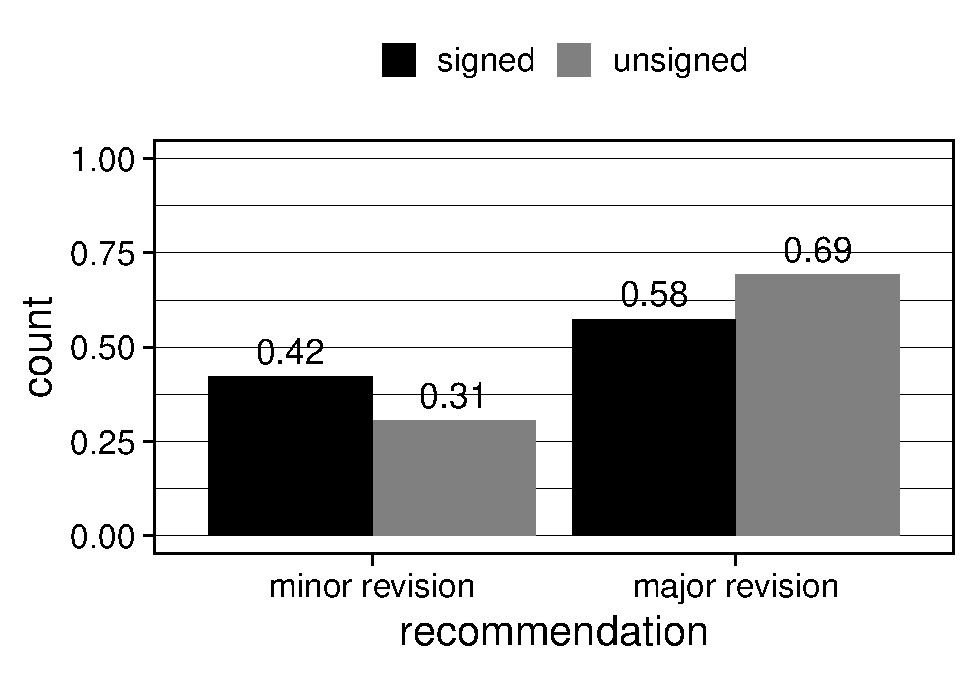
\includegraphics{open_peer_review_files/figure-latex/PeerJrec-1.pdf}
\caption{\label{fig:PeerJrec}Frequencies of signed and unsigned reviews as a function of whether the handling editor at PeerJ recommended \enquote{minor revisions} or \enquote{major revisions}.}
\end{figure}

Analyzing the reviews at the Royal Society provides a more direct answer to our question, since each individual reviewer is asked to provide a recommendation of \enquote{accept}, \enquote{minor revisions}, \enquote{major revisions}, or \enquote{reject}. We can therefore directly compare how recommendations are related to the decision to sign reviews. The percentage of signed peer reviews is decreases as recommendations become more negative, from 46.99\% for \enquote{accept} recommendations, 43.86\% for \enquote{minor revisions}, 29.48\% for \enquote{major revisions}, and 11.07\% for \enquote{reject} recommendations.

Since these data are correlational we can not draw causal conclusions. It is possible that reviewers are less likely to sign more negative reviews. It is also possible that people who sign their reviews are in general less negative in their recommendations, and therefore the distribution of signed reviews differs from non-signed reviews. Given the literature described in the introduction that provides anecdotal evidence researchers worry they will be able to provide open criticism if their names are public, and experimental evidence suggesting that if names are made public, recommendation become somewhat more positive, it seems plausible at least part of the pattern we observed can be explained by reviewers being more likely to sign their more positive reviews.

\hypertarget{additional-analyses}{%
\section{Additional Analyses}\label{additional-analyses}}

Open reviews make it possible to examine additional interesting questions. The dataset we are sharing has information about the recommendations of reviewers or editors after each round of peer review, and the names of reviewers who signed their review. Through the DOI, researchers can link this data to, for example, citation counts for each manuscript. This makes it possible to explore whether initial evaluations of a manuscript are related to future citations counts. By manually coding which career stage authors and reviewers belong to during the review process it is possible to gain insights into who is more likely practice open science. Because the reviews themselves are included in our dataset, researchers interested can use the text files to answer more details questions about the content of peer reviews across different domains.

For example, since multiple reviewers for The Royal Society Open Science and Open Biology make their individual recommendations known, we can see how often reviewers agree. For the 1559 individual papers that we were able to retrieve reviews from, reviewers agreed on the recommendation in 646 (41.44\%) of the time. For 42.14\% of the manuscripts the maximum deviation was one category (e.g., minor and major revisions), for 14.69\% of the manuscripts the maximum deviation was two categories (e.g., accept and major revision), and for 1.73\% of the manuscripts the maximum deviation was three categories (i.e., accept and reject). There were 3 articles where researchers received all four possible recommendations (accept, minor revisions, major revisions, reject) from at least four different reviewers.

The average time between submission and acceptance for PeerJ for the articles open reviews are available for was 112 days, and for the Royal Society this was 133 days.

\begin{figure}
\centering
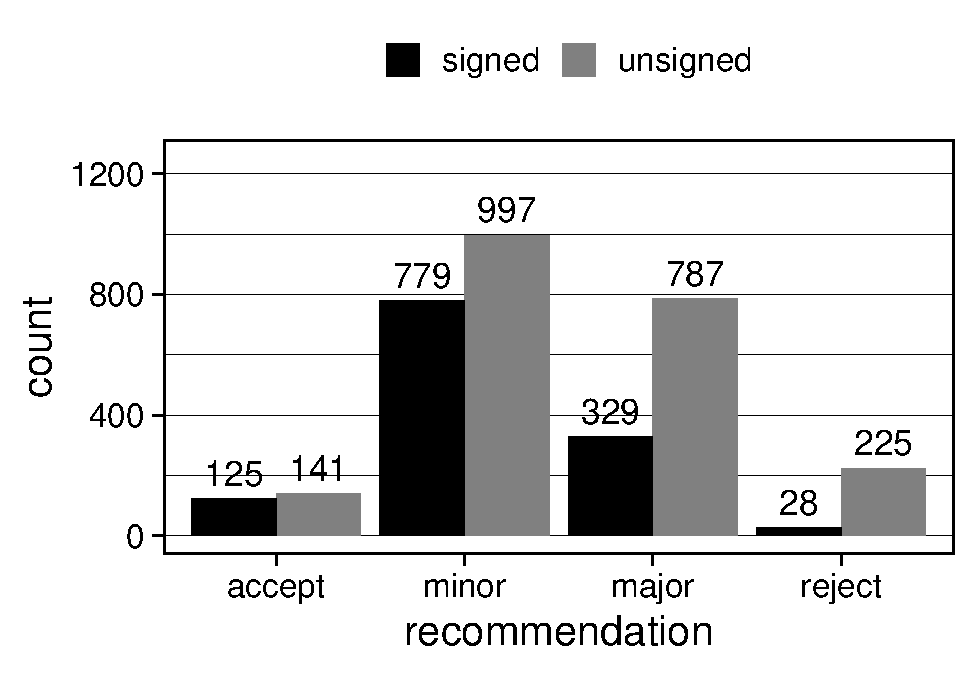
\includegraphics{open_peer_review_files/figure-latex/TRSrec-1.pdf}
\caption{\label{fig:TRSrec}Frequencies of signed and unsigned reviews as a function of whether the reviewer at the Royal Society Open Science and Open Biology recommended \enquote{accept}, \enquote{minor revisions}, \enquote{major revisions}, or \enquote{reject}.}
\end{figure}

\begin{verbatim}
## 
##  2-sample test for equality of proportions with continuity
##  correction
## 
## data:  prop_data
## X-squared = 142.6, df = 1, p-value < 2.2e-16
## alternative hypothesis: two.sided
## 95 percent confidence interval:
##  -0.1369924 -0.0978543
## sample estimates:
##    prop 1    prop 2 
## 0.5362998 0.6537231
\end{verbatim}

\begin{verbatim}
## [1] 0.6000000 0.5362998 0.6537231
\end{verbatim}

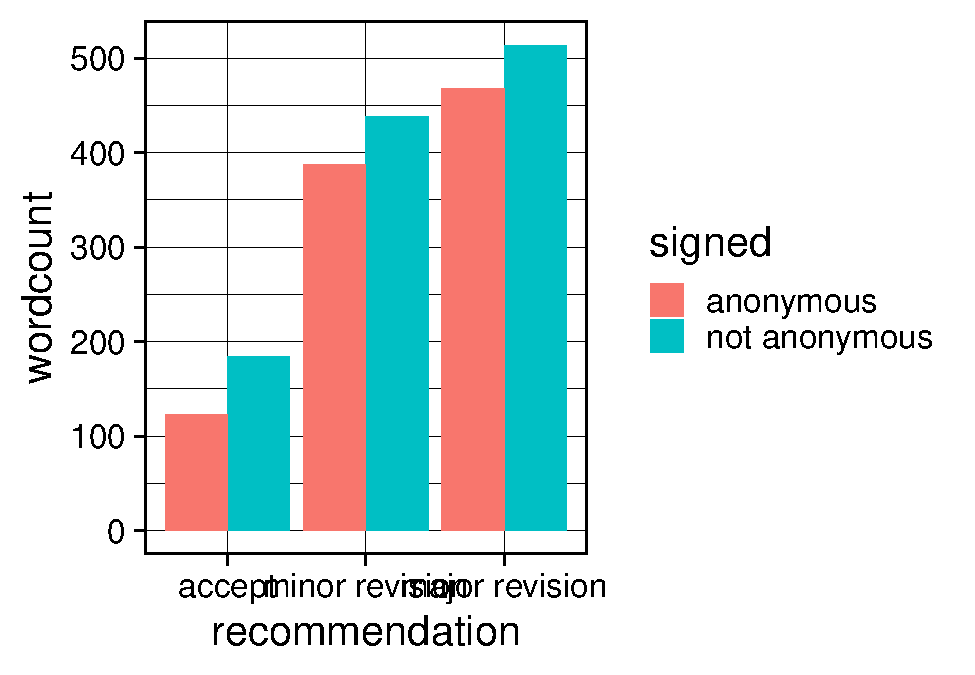
\includegraphics{open_peer_review_files/figure-latex/unnamed-chunk-3-1.pdf}

\begin{verbatim}
## Warning: Removed 2 rows containing missing values (geom_bar).
\end{verbatim}

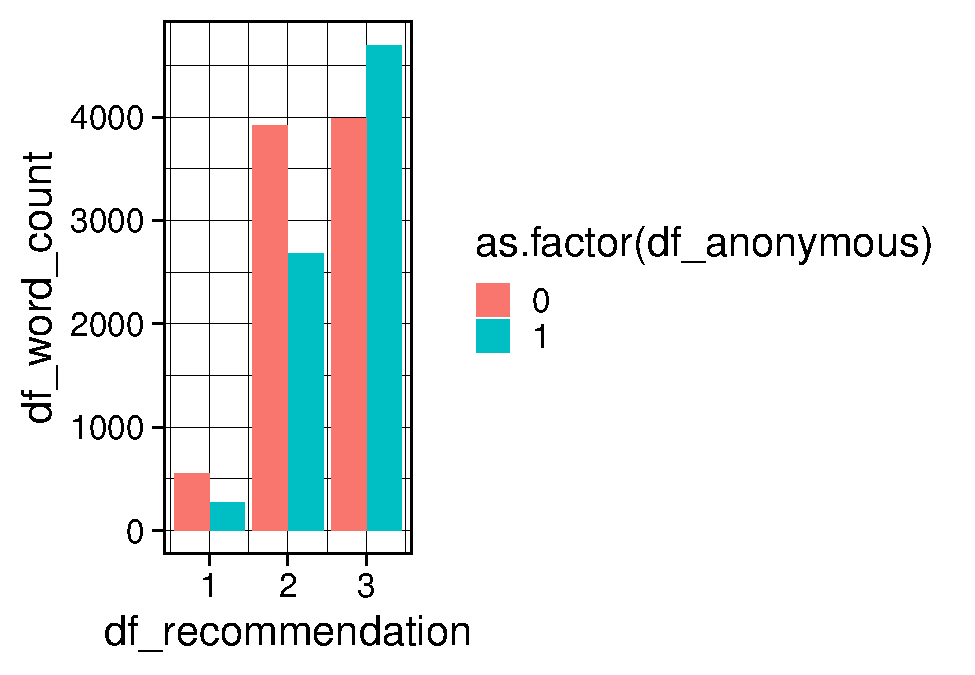
\includegraphics{open_peer_review_files/figure-latex/unnamed-chunk-3-2.pdf}

\begin{verbatim}
## Warning: Removed 2 rows containing missing values (geom_point).
\end{verbatim}

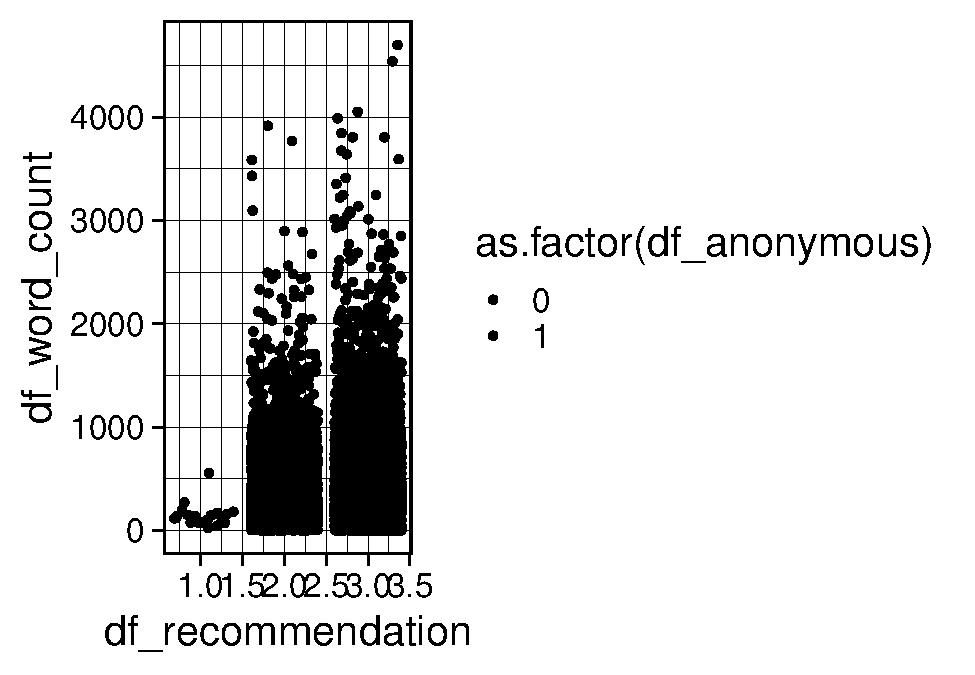
\includegraphics{open_peer_review_files/figure-latex/unnamed-chunk-3-3.pdf}

\begin{verbatim}
## 
##  Welch Two Sample t-test
## 
## data:  PeerJ_data_R1$df_word_count by PeerJ_data_R1$df_anonymous
## t = 4.3438, df = 8046.6, p-value = 1.418e-05
## alternative hypothesis: true difference in means is not equal to 0
## 95 percent confidence interval:
##  21.25429 56.21419
## sample estimates:
## mean in group 0 mean in group 1 
##        481.1711        442.4369
\end{verbatim}

In Nino's BEP there were 3552 reviews in RSOS. I have 3629 after running all his code.

Older Royal Society journals have the comment: Note: This manuscript was transferred from another Royal Society journal without peer review.
What does this mean?

Word counts are not perfectly reliable for several reasons (e.g., addition of references, but also more importantly comments in an attached pdf - maybe we can search for attached and pdf in short comments to identify these. )

" This result is similar to the findings in Bornmann, Wolf,
and Daniel (2012) that the comments in public peer review are much longer than
the comments in closed peer review."

\hypertarget{future-research}{%
\subsection{Future Research}\label{future-research}}

\hypertarget{notes}{%
\subsection{NOTES}\label{notes}}

Searching all text files of PeerJ for \enquote{appealed on} reveals 44 articles that were initially appealed, and subsequently published.
From Nino's thesis for RSOS: \enquote{Interestingly, for 39 of the reviews we had
access to (and were thus published) the final recommendation given by the editor is to reject the manuscript. For these articles to still get published, the author has to appeal the rejection and change the decision made by the editor.}
Not sure how he got this - my code does not suggest this.
sum(PeerJ\_data\$df\_recommendation == 4, na.rm = TRUE) \# how many reviews for first submissions

From Wang et al: " Of the 3,569 review reports, 85 were submitted as
attachments in various formats (comments inserted to the manuscripts, PDF or Word
DOC) or the reviews contained no substantive content such as \enquote{no further comments.}"

\hypertarget{author-contributions}{%
\section{Author Contributions}\label{author-contributions}}

N. van Sambeek and D. Lakens developed the idea. Both authors generated the R code to generate the data and anayze the results. N van Sambeek drafted the initial version of the manuscript as a Bachelor thesis, D. Lakens wrote the final version, both authors revised the manuscript.

\hypertarget{conflict-of-interest-statement}{%
\section{Conflict of Interest Statement}\label{conflict-of-interest-statement}}

The authors report no conflicts of interest.

\hypertarget{references}{%
\section{References}\label{references}}

\setlength{\parindent}{-0.5in}
\setlength{\leftskip}{0.5in}

\hypertarget{refs}{}
\leavevmode\hypertarget{ref-mulligan_peer_2013}{}%
Mulligan, A., Hall, L., \& Raphael, E. (2013). Peer review in a changing world: An international study measuring the attitudes of researchers. \emph{Journal of the American Society for Information Science and Technology}, \emph{64}(1), 132--161. doi:\href{https://doi.org/10.1002/asi.22798}{10.1002/asi.22798}

\leavevmode\hypertarget{ref-ooms_pdftools_2019}{}%
Ooms, J. (2019). \emph{Pdftools: Text extraction, rendering and converting of PDF documents}.

\leavevmode\hypertarget{ref-rooyen_effect_2010}{}%
Rooyen, S. van, Delamothe, T., \& Evans, S. J. W. (2010). Effect on peer review of telling reviewers that their signed reviews might be posted on the web: Randomised controlled trial. \emph{BMJ}, \emph{341}, c5729. doi:\href{https://doi.org/10.1136/bmj.c5729}{10.1136/bmj.c5729}

\leavevmode\hypertarget{ref-ross-hellauer_survey_2017}{}%
Ross-Hellauer, T., Deppe, A., \& Schmidt, B. (2017). Survey on open peer review: Attitudes and experience amongst editors, authors and reviewers. \emph{PLOS ONE}, \emph{12}(12), e0189311. doi:\href{https://doi.org/10.1371/journal.pone.0189311}{10.1371/journal.pone.0189311}

\leavevmode\hypertarget{ref-walsh_open_2000}{}%
Walsh, E., Rooney, M., Appleby, L., \& Wilkinson, G. (2000). Open peer review: A randomised controlled trial. \emph{The British Journal of Psychiatry}, \emph{176}(1), 47--51. doi:\href{https://doi.org/10.1192/bjp.176.1.47}{10.1192/bjp.176.1.47}

\leavevmode\hypertarget{ref-wang_open_2016}{}%
Wang, P., You, S., Manasa, R., \& Wolfram, D. (2016). Open peer review in scientific publishing: A Web mining study of PeerJ authors and reviewers. \emph{Journal of Data and Information Science}, \emph{1}(4), 60--80.

\leavevmode\hypertarget{ref-wickham_stringr_2019}{}%
Wickham, H. (2019). \emph{Stringr: Simple, consistent wrappers for common string operations}.


\end{document}
